%%%%%%%%%%%%%%%%%%%%%%%%%%%%%%%%%%%%%%%%%%%%%%%%%%%%%%%%%%%%%%%%%%%%%%%%
%                                                                      %
%     File: Thesis_Background.tex                                      %
%     Tex Master: Thesis.tex                                           %
%                                                                      %
%     Author: Andre C. Marta                                           %
%     Last modified :  4 Mar 2024                                      %
%                                                                      %
%%%%%%%%%%%%%%%%%%%%%%%%%%%%%%%%%%%%%%%%%%%%%%%%%%%%%%%%%%%%%%%%%%%%%%%%

\chapter{Theoretical Background}
\label{chapter:background}

In this chapter, we cover the theoretical background necessary for understanding the subsequent material of this work. We start by discussing the well-posedness of Cauchy problems in systems of partial differential equations in section \ref{section:well-posedness}, which is a necessary condition for our models to have predictive power. We then introduce the 3+1 formalism in section \ref{section:3+1_formalism}, which allows us to separate spacetime into three-dimensional space and time, making it easier to study the dynamical evolution of gravitational fields. Next, we discuss hyperboloidal compactification in section \ref{section:compactification}, a technique that enables us to study the asymptotic behavior of solutions at future null infinity. Finally, we present the wave equation and its cubic non linearity in the sections \ref{section:wave_equation} and \ref{section:cubic_wave_equation} respectively, which are the central objects of our study.


%%%%%%%%%%%%%%%%%%%%%%%%%%%%%%%%%%%%%%%%%%%%%%%%%%%%%%%%%%%%%%%%%%%%%%%%
\section{Well-Posedness of Cauchy Problems in Systems of PDEs}
\label{section:well-posedness}

When dealing with systems of partial differential equations, one generally works with initial value problems (also sometimes called \textit{Cauchy problems}), which consist of, given initial data $u(0,x^i) = f(x^i)$ at a time $t = 0$, calculating the solution $u(t,x^i)$ for a later time. These problems are very relevant in physics due to the predictive character of our models. However, for our systems to possess this predictive power, they must be \textit{well-posed}. \textit{Well-posedness} in a partial differential equation problem is the requirement that there be a unique solution that depends continuously, in some norm, on the given data for the problem \cite{AN_INTRODUCTION_TO_WELLPOSEDNESS_AND_FREEEVOLUTION}. More rigorously, we say an initial value problem is well-posed if there exist constants $K$ and $\alpha$ such that
%
\begin{align}
 ||u(t,\, \cdot)||_{L^2} 
     \leq K e^{\alpha t} ||f||_{L^2},
\end{align}
%
where the initial data of the \textit{Cauchy problem} is given by $u(0,x^i) = f(x^i)$ and the $L^2$ norm is given by
%
\begin{align}
    ||g||_{L^2}^2 = \int_{\mathbb{R}^3} g^\dagger\, g \; dV.
\end{align}

Without this property, small changes in the given data may result in arbitrarily large changes in the solution or render it impossible to find a solution at all. Thus, we must make sure to formulate our field equations in such a way that they form a well-posed system of differential equations.

Let us consider a system of partial differential equations that can be written as
%
\begin{align}
    \partial_t u = A^p \partial_p u + B \, u,
    \label{eq:strong_hyp}
\end{align}
%
where $u$ is a state vector. We call $A^p$ the \textit{principal matrix} of the system despite it being an abbreviation for three matrices (one for each spatial dimension). The remaining terms on the right-hand side of our system of differential equations non-principal \cite{AN_INTRODUCTION_TO_WELLPOSEDNESS_AND_FREEEVOLUTION}. Given an arbitrary unit spatial vector $s^i$, we define the \textit{principal symbol} of the system as
%
\begin{align}
    P^s \equiv A^s = A^p s_p.
\end{align}

If, for every unit spatial vector $s^i$, the \textit{principal symbol} of our system has real eigenvalues, our system is considered \textit{weakly hyperbolic}. If, in addition to our system being \textit{weakly hyperbolic}, we have that for every unit spatial vector $s^i$, the principal symbol has a complete set of eigenvectors, and there exists a constant $K$, independent of $s^i$, such that
%
\begin{align}
    ||T_s|| + ||T_s^{-1}|| \leq K,
\end{align}
%
where $T_s$ is a matrix that has the eigenvectors of $P^s$ as columns and we have the usual definition of the matrix norm $||\cdot||$; we call our system \textit{strongly hyperbolic}. The components of the vector $v = T^{-1}_s u$ are called \textit{characteristic variables} in the $s^i$ direction, which satisfy advection equations with speeds equal to the eigenvectors of the principal symbol up to non-principal terms and derivatives transverse to the $s^i$ direction. In other words, they satisfy equation \eqref{eq:strong_hyp} along the $s^i$ direction. These variables will be relevant when we discuss how \texttt{bamps} handles patch boundaries in section \ref{section:Patch_Boundaries}.


Let us now consider a system of partial differential equations written as
\begin{align}
    \partial_t u = A^p \partial_p u + F(t,x^i),
\end{align}
%
where we only consider solutions on the half-space $x^1 = x\geq 0$, making it so that we have a boundary. We call $F$ the forcing term, which could be, for example, $F = B \, u$ as in equation \eqref{eq:strong_hyp}. In this initial value problem, we provide initial conditions for the domain $u(0,x^i)=f(x^i)$, and boundary conditions $L\, u(t,x^i) \stackrel{\wedge}{=} g(t,x^A)$, where the index $A$ denotes that the data depends only on $x^2 = y$ and $x^3=z$, with $L$ a matrix that will be described later, and $\stackrel{\wedge}{=}$ denotes equality on the boundary.

We say that our system is \textit{symmetric hyperbolic} if there exists a Hermitian positive definite symmetrizer $H$ such that $H A^p s_p$ is Hermitian for every spatial vector $s_p$. This property of a system is very relevant as it is related to \textit{strong well-posedness} when the boundaries of our system are \textit{maximally dissipative}, as we will see briefly. It is important to note that every \textit{symmetric hyperbolic} system is \textit{strongly hyperbolic}, even though the opposite is not true.

Saying that an initial value problem is \textit{strongly well-posed} means that we can bind the solution in the bulk and restrict it to the initial boundary data with the addition of growth caused by non-principal terms or the boundaries \cite{AN_INTRODUCTION_TO_WELLPOSEDNESS_AND_FREEEVOLUTION}. That is, an initial value problem is \textit{strongly well-posed} if, for every time $T$, there exists a constant $K_T$ independent of the initial data and the forcing terms such that, for $0 \leq t \leq T$, we have
%
\begin{align}
 ||u(t,\cdot)||^{2}_\Sigma + \int_{0}^{t} ||u(t',\cdot)||^{2}_{\partial \Sigma} \; dt' 
     \leq K_{T}^{2} \Bigg( ||f|^{2}_\Sigma + \int_{0}^{t} \Big(||F(t',\cdot)||^{2}_\Sigma + ||g(t',\cdot)||^{2}_{\partial \Sigma} \Big) dt' \Bigg),
\end{align}
%
where $||\cdot||_\Sigma$ denotes the $L^2$ norm on the half-space, and $||\cdot||_{\partial \Sigma}$ denotes the $L^2$ norm on the boundary plane.

Since every \textit{symmetric hyperbolic} system is \textit{strongly hyperbolic}, there exists a matrix $T_x$ such that
%
\begin{align}
 T_x^{-1}P^x T_x = \Lambda_x = 
    \begin{pmatrix} 
        \Lambda_x^I & 0 \\
        0 & \Lambda_x^{II} 
    \end{pmatrix}.
\end{align}

If we have $\Lambda_I > 0$ and $\Lambda_{II} < 0$, our system has \textit{maximally dissipative} boundaries. If those conditions are not met, our system has characteristic boundaries in the variables where the characteristic speed vanishes at the boundaries.

We can prove the \textit{well-posedness} of our initial value problem by defining the energy
%
\begin{align}
 E = \int_\Sigma \epsilon \; dV = \int_\Sigma u^\dagger H u \; dV \; .
\end{align}
%
By taking the time derivative of this energy and performing an integration by parts, we get
%
\begin{align}
  \partial_t E + c_1 \int_{\partial\Sigma} \left( u^\dagger H u \right) \; dS 
    \leq \int_\Sigma \left( u^\dagger H F + F^\dagger H u \right) \; dV + c_2 \int_{\partial \Sigma} \left( g^\dagger H g\right) \; dS ,
\end{align}
%
for some $c_1, c_2 > 0$, from which we get \textit{strong well-posedness} \cite{AN_INTRODUCTION_TO_WELLPOSEDNESS_AND_FREEEVOLUTION}. It is important to note that \textit{maximally dissipative} boundary conditions only guarantee \textit{well-posedness} for \textit{symmetric hyperbolic} systems, not for \textit{strongly hyperbolic} ones.

%%%%%%%%%%%%%%%%%%%%%%%%%%%%%%%%%%%%%%%%%%%%%%%%%%%%%%%%%%%%%%%%%%%%%%%%
\section{The 3+1 Formalism}
\label{section:3+1_formalism}

One usually finds the Einstein field equations written in a fully covariant form, where there isn't a clear distinction between space and time. However, in numerical relativity, we are interested in studying the dynamical evolution of a gravitational field in "time". It is thus convenient to split spacetime into three-dimensional space and time. That way, we can provide spacelike initial conditions and obtain the subsequent evolution along our time coordinate. To perform that separation, we use the so-called 3+1 Formalism \cite{3+1_Formalism_and_Bases_of_Numerical_Relativity,Introduction_to_3+1_numerical_relativity,Numerical_Relativity_Solving_Einsteins_Equations_on_the_Computer}.

We start by considering a spacetime with the metric $g_{ab}$~. To maintain hyperbolicity in our evolution equations, we must restrict our spacetimes to be globally hyperbolic, meaning they possess a Cauchy surface. These globally hyperbolic spacetimes can be completely foliated in a way such that each three-dimensional slice is spacelike. Additionally, we can identify each three-dimensional hypersurface with the level set of a parameter $t$~, which we consider to be a universal time function. 

Given two adjacent hypersurfaces $\Sigma_t$~and $\Sigma_{t+dt}$~in a specific foliation, we can determine the geometry of the region of spacetime between them by studying the movement of observers moving along the direction normal to the hypersurfaces. We call those observers \textit{Eulerian}. Considering those observers, we define three quantities that can describe our region of interest: the three-dimensional metric $\gamma_{ij}$~(which measures proper distances within the hypersurfaces), the lapse function $\alpha$~(which is the lapse of proper time between both hypersurfaces measured by \textit{Eulerian observers}), and the shift vector $\beta^i$~(which is the relative velocity between the \textit{Eulerian observers} and the lines of constant spatial coordinates). It is also useful to define the extrinsic curvature $K_{\mu\nu}$~(which measures the change of the normal vector to the hypersurface when parallel transported from one point in the hypersurface to another) and the acceleration of the \textit{Eulerian observers} $a^i$ \cite{3+1_Formalism_and_Bases_of_Numerical_Relativity,Introduction_to_3+1_numerical_relativity,Numerical_Relativity_Solving_Einsteins_Equations_on_the_Computer}.

\begin{figure}[t!]
\centering
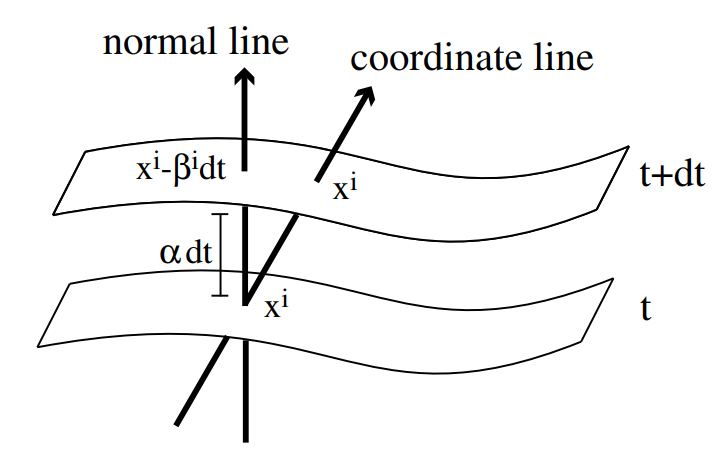
\includegraphics[width=0.5\textwidth]{Figures/Definitions_of_the_3+1_quantities.png}
\caption{Geometric definition of the lapse function $\alpha$ and the shift vector $\beta^i$. The lapse function $\alpha$ is the proper time between two adjacent hypersurfaces $\Sigma_t$ and $\Sigma_{t+dt}$ measured by \textit{Eulerian observers}. The shift vector $\beta^i$ is the relative velocity between the \textit{Eulerian observers} and the lines of constant spatial coordinates. \cite{Introduction_to_3+1_numerical_relativity}}
\end{figure}

In this work, we are interested in specifying initial conditions starting from a known spacetime metric $g_{ab}$~. Thus, we need to calculate the previously mentioned 3+1 quantities from $g_{ab}$~, which can be done by performing a 3+1 split of $g_{ab}$~. This split is done by writing $g_{ab}$~as a function of $\alpha$~, $\beta^i$~and $\gamma_{ij}$~:
%
\begin{align}
 ds^2 = (-\alpha^2 + \beta_i \beta^i) ~ dt^2 
     + 2 \beta_i ~ dt dx^i 
     + \gamma_{ij} ~ dx^i dx^j,
\end{align}
%
or, more explicitly,
%
\begin{align}
    \begin{aligned}
        g_{\mu\nu} = \begin{pmatrix} 
            -\alpha^2 + \beta_k \beta^k & \beta_i \\
            \beta_j & \gamma_{ij} 
        \end{pmatrix}, 
        & \quad \quad \quad 
        g^{\mu\nu} = \begin{pmatrix} 
            -1/\alpha^2 & \beta^i/\alpha^2 \\
            \beta^j/\alpha^2 & \gamma^{ij} - \beta^i \beta^j/\alpha^2
        \end{pmatrix}.
    \end{aligned}
\end{align}

Using this split, it becomes easy to obtain $\alpha$~, $\beta^i$~and $\gamma_{ij}$~from $g_{ab}$~, from which we can obtain the extrinsic curvature $K_{\mu\nu}$~using the fact that
%
\begin{align}
 K_{ij} = \frac{D_i \beta_j + D_j \beta_i - \partial_t \gamma_{ij}}{2 \alpha},
\end{align}
%
where $D_\mu := (\delta^\alpha_\mu + n^\alpha n_\mu) \nabla_\alpha$~is the projection of the covariant derivative onto the hypersurface and $n$~is the normal vector to the hypersurface, with components given by
%
\begin{align}
    \begin{aligned}
        n^\mu = (1/\alpha,~-\beta^i/\alpha), 
        & \quad \quad \quad n_\mu = (-\alpha,~0).
    \end{aligned}
\end{align}

We can also obtain the acceleration of the \textit{Eulerian observers} $a^i$~as
\begin{align}
 a^i = \gamma^{ij} \partial_j(\ln \alpha).
\end{align}


%%%%%%%%%%%%%%%%%%%%%%%%%%%%%%%%%%%%%%%%%%%%%%%%%%%%%%%%%%%%%%%%%%%%%%%%
\section{Hyperboloidal Compactification}
\label{section:compactification}

In this work, we are interested in studying how waves behave at future null infinity, making it useful to compactify our spacetime in such a way that allows us to study the asymptotic behavior of our solutions numerically. To accomplish this, we will employ a specific set of coordinates called \textit{hyperboloidal coordinates} \cite{Hyperboloidal_layers_for_hyperbolic_equations_on_unbounded_domains,The_evolution_of_hyperboloidal_data_with_the_dual_foliation_formalism_Mathematical_analysis_and_wave_equation_tests}. 

The hyperboloidal coordinates $(t, r)$ are related to the usual spherical coordinates $(T, R)$ by the \textit{height function} $H(R)$~and the \textit{compress function} $\Omega(r)$~as follows:
%
\begin{align}
 T = t + H(R), 
     \quad \quad \quad R = \Omega^{-1}(r) \, r.
\end{align}
%
The angular coordinates remain unchanged. This transformation gives rise to the Jacobian matrix
%
\begin{align}
    \left(J^{Hyp}\right)_{\alpha'}^{\ \ \beta} = 
    \begin{pmatrix}
        1 & -H'(r) & 0 & 0 \\
        0 & \frac{L(r)}{\Omega^2(r)} & 0 & 0 \\
        0 & 0 & 1 & 0 \\
        0 & 0 & 0 & 1
    \end{pmatrix} \; ,
\end{align}
%
where $H'(r)$ denotes the derivative of the height function with respect to $R$ written as a function of $r$, and $L(r)$ is defined as
%
\begin{align}
 L(r) \equiv \Omega(r) - r \, \partial_r \Omega(r) \; .
\end{align}

It is important to note that, even though there is freedom to choose the height and the compress function, we must require that, asymptotically in $R$, or equivalently, as $\Omega$ approaches zero, we have
%
\begin{align}
    1 - H' \sim O(\Omega^2) \, .
\end{align}

Since the solutions to our equations decay as we approach null infinity, it is useful to rescale our spacetime in such a way that our solutions are of order one through space. Given a spacetime with metric $g_{ab}$~, we can rescale it by a strictly positive, smooth scalar function $\Omega$~to obtain a new metric $\tilde{g}_{ab}$~:
%
\begin{align}
    \tilde{g}_{ab} = \Omega^2 g_{ab},
\end{align}
%
This rescaling is called a \textit{conformal transformation} and the function $\Omega$~ is called the \textit{conformal factor}. If $g_{ab}$~is a Lorentzian metric, then a vector $v^a$~is timelike, null or spacelike with respect to $g_{ab}$~ if and only if it is timelike, null or spacelike with respect to $\tilde{g}_{ab}$~, meaning that the causal structure of the spacetime is preserved under conformal compactification \cite{wald:1984}. 

After applying both the coordinate transformation to hyperboloidal coordinates and the conformal transformation, we obtain a new metric $\tilde{g}_{ab}$~, which on Cartesian coordinates is given by

\begin{align}
    \tilde{g}_{ab} = 
    \begin{pmatrix}
        -\Omega^2(r) & -\frac{x H(r) L(r)}{r} & -\frac{y H(r) L(r)}{r} & -\frac{z H(r) L(r)}{r} \\
        -\frac{x H(r) L(r)}{r} & \frac{(y^2 + z^2) \mathcal{R}^2(r) + r^2 x^2 L^2(r) \Xi(r)}{r^4} & \frac{x y (-\mathcal{R}^2(r) + r^2 L^2(r) \Xi(r))}{r^4} & \frac{x z (-\mathcal{R}^2(r) + r^2 L^2(r) \Xi(r))}{r^4} \\
        -\frac{y H(r) L(r)}{r} & \frac{x y (-\mathcal{R}^2(r) + r^2 L^2(r) \Xi(r))}{r^4} & \frac{(x^2 + z^2) \mathcal{R}^2(r) + r^2 y^2 L^2(r) \Xi(r)}{r^4} & \frac{y z (-\mathcal{R}^2(r) + r^2 L^2(r) \Xi(r))}{r^4} \\
        -\frac{z H(r) L(r)}{r} & \frac{x z (-\mathcal{R}^2(r) + r^2 L^2(r) \Xi(r))}{r^4} & \frac{y z (-\mathcal{R}^2(r) + r^2 L^2(r) \Xi(r))}{r^4} & \frac{(x^2 + y^2) \mathcal{R}^2(r) + r^2 z^2 L^2(r) \Xi(r)}{r^4}
    \end{pmatrix} \; ,
\end{align}
%
where we have defined $\Xi(r)$ and $\mathcal{R}(r)$ as
%
\begin{align}
    \Xi(r) = \frac{1 - H^2(r)}{\Omega^2(r)} \; , \quad \quad \quad \mathcal{R}(r) = r - R_i + R_i \Omega(r) \; ,
\end{align}
%
with $R_i$ being the interface radius, which we will now briefly discuss.

In some applications, it may be useful to consider a flat slice where most of the dynamics happen, followed by a hyperboloidal slice, which allows us to study the decay of our solution as it approaches future null infinity \cite{Hyperboloidal_layers_for_hyperbolic_equations_on_unbounded_domains,The_evolution_of_hyperboloidal_data_with_the_dual_foliation_formalism_Mathematical_analysis_and_wave_equation_tests}. That scenario can be achieved using \textit{hyperboloidal layers}, which consist of performing a transition from flat slices to hyperboloidal slices at a chosen interface radius $R_i$, making it such that we achieve a hyperboloidal slice after some transition length $l_t$. The details of this transition will be further discussed in section \ref{section:hyp_layers_wave}.


%%%%%%%%%%%%%%%%%%%%%%%%%%%%%%%%%%%%%%%%%%%%%%%%%%%%%%%%%%%%%%%%%%%%%%%%
\section{The Wave Equation}
\label{section:wave_equation}

The wave equation is a symmetric hyperbolic partial differential equation that describes the propagation of all types of wave-like phenomena. In the study of gravitational waves, this equation is of particular importance due to its structural similarity to the Einstein field equations on the \textit{Generalized Harmonic Gauge (GHG)}. The wave equation, in its simpler form, is given by
%
\begin{align}
    \Box_g \Psi = S,
    \label{eq:wave_equation_simple}
\end{align}
%
where $\Box_g$ is the d'Alembert operator, $\Psi$ is the scalar field, and $S$ is a source term. The Einstein equations in the GHG can be written as
%
\begin{align}
    \Box_g g_{ab} = 2 g^{cd} g^{ef} (\partial_e g_{ca} \partial_f g_{db} - \Gamma_{ace} \Gamma_{bdf}),
\end{align}
%
where $g_{ab}$ is the spacetime metric, $\Gamma_{abc}$ are the Christoffel symbols, and $g^{ab}$ are the inverse metric \cite{A_new_generalized_harmonic_evolution_system}. The similarity between these two equations allows us to study the wave equation as a model for gravitational waves.

It is important to note that when we perform a conformal transformation of the spacetime like the one described in section \ref{section:compactification}, the d'Alembert operator in the new metric $\tilde{g}_{ab}$~becomes
%
\begin{align}
    \Box_{\tilde{g}} \tilde{\psi} = \tilde{g}^{ab} \tilde{\nabla}_a \tilde{\nabla}_b \tilde{\psi}
    &= \Omega^{s-2} g^{ab} \nabla_a \nabla_b \psi + s \Omega^{s-3} \psi\, g^{ab} \nabla_a \nabla_b \Omega \\
    &\quad + s(n + s - 3) \Omega^{s-4} \psi\, g^{ab} \nabla_a \Omega \nabla_b \Omega
    \label{eq:conformal_wave_equation1}
\end{align}
%
where $s$~is the conformal weight of the scalar field $\psi$ (which we can choose freely)~and $n$~is the dimension of the spacetime \cite{wald:1984}. In this work, we will be working in a four-dimensional spacetime, so $n = 4$~. The conformal weight $s$~will be chosen to be $s = -1$ to simplify the expression of equation \eqref{eq:conformal_wave_equation1}. Thus, we have
%
\begin{align}
    \tilde{g}^{ab} \tilde{\nabla}_a \tilde{\nabla}_b \tilde{\psi} 
 =&~\Omega^{-3} g^{ab} \nabla_a \nabla_b \psi 
 - \Omega^{-4} \psi\, g^{ab} \nabla_a \nabla_b \Omega,
    \label{eq:conformal_wave_equation2}
\end{align}
%
We can now substitute \eqref{eq:wave_equation_simple} into \eqref{eq:conformal_wave_equation2} and write the resulting equation in terms of the rescaled quantities, obtaining
%
\begin{align}
    \tilde{g}^{ab} \tilde{\nabla}_a \tilde{\nabla}_b \tilde{\psi} 
 =&~\Omega^{-3} S 
 - \Omega^{-1} \tilde{\psi} \bigg( 
    \tilde{g}^{ab} \tilde{\nabla}_a \tilde{\nabla}_b \Omega 
 - 2 \Omega^{-1} \tilde{g}^{ab} \tilde{\nabla}_a \Omega \tilde{\nabla}_b \Omega \bigg),
\end{align}
%
which is the wave equation for the rescaled scalar field $\tilde{\psi}$~in the compactified spacetime with metric $\tilde{g}_{ab}$~.

To solve the previous equation numerically, it is useful to do a 3+1 decomposition of spacetime and write the system as a set of first-order partial differential equations. To do that, we start by employing the 3+1 split of the metric $\tilde{g}_{ab}$~described in section \ref{section:3+1_formalism} and define the time reduction variable $\tilde{\Pi}$~and the spatial reduction variables $\tilde{\phi}_i$~as
%
\begin{align}
    \Pi = - \mathcal{L}_n \tilde{\psi} \;  \quad \quad \quad \phi_i = \tilde{D}_i \tilde{\psi} \; ,
\end{align}
%
where $\mathcal{L}_n$~is the Lie derivative along the normal vector to the hypersurface $n^a$~, and $\tilde{D}_i$~is the projection of the covariant derivative onto the hypersurface. It is important to note that these definitions introduce new constraints to our system, given by
%
\begin{align}
    \begin{cases}
        \mathcal{L}_n \tilde{\psi} + \Pi \overset{!}{=} 0 \\
        \tilde{D}_i \tilde{\psi} - \phi_i \overset{!}{=} 0
    \end{cases}\,,
\end{align}
%
where $\overset{!}{=}$ denotes that we may allow for small violations of these constraints due to numerical errors. The second constraint is of particular importance as we will see later in section \ref{section:hyp_wave}. Due to this importance, we will denote it as $C_i$.

Using the previous definitions, we can write the wave equation as a set of first-order partial differential equations as
%
\begin{align}
    \begin{cases}
        \partial_t \tilde{\psi} = - \tilde{\alpha} \tilde{\Pi} + \beta^i \tilde{\phi}_i \\
        \partial_t \tilde{\phi}_i = - \tilde{\alpha} (\tilde{D}_i \tilde{\Pi}) - (\tilde{D}_i \tilde{\alpha}) \tilde{\Pi} + \beta^j \partial_j \tilde{\phi}_i + \tilde{\phi}_j \partial_i \beta^j \\
        \partial_t \tilde{\Pi} = - \tilde{\alpha} \tilde{a}^i \tilde{\phi}_i - \tilde{\alpha} \tilde{\gamma}^{ij} \tilde{D}_j \tilde{\phi}_i + \tilde{\alpha} \tilde{K} \tilde{\Pi} + \beta^i \tilde{D}_i \tilde{\Pi} \\
        \hspace{3.5em} - \tilde{\alpha} \Omega^{-1} \Big( \tilde{g}^{ab} \tilde{\nabla}_a \tilde{\nabla}_b \Omega - 2 \Omega^{-1} \tilde{g}^{ab} \tilde{\nabla}_a \Omega \tilde{\nabla}_b \Omega \Big) \tilde{\psi} + \tilde{\alpha} \Omega^{-3} S
    \end{cases}\,.
    \label{eq:wave_equation_3+1}
\end{align}

It is also necessary to calculate the characteristic variables of our system and their respective speeds. To do so, we start by calculating the principal symbol of our system and its eigenvalues, obtaining advection equations for the characteristic variables
%
\begin{align}
    \begin{cases}
        \partial_t \tilde{\psi} = 0 \\
        \partial_t (\tilde{\Pi} \pm \tilde{\phi}_s) = - (-\beta^s \pm \tilde{\alpha}) \partial_s (\tilde{\Pi} \pm \tilde{\phi}_s)
    \end{cases}\,,
\end{align}
%
where $\tilde{\phi}_s = \tilde{\phi}_i s^i$~(it is important to note that this definition does not let~$\tilde{\phi}_i$~and~$s^i$~commute) and similarly for $\beta^s$, with $s^i$~being an arbitrary unit spatial vector. From this, we can identify the characteristic variables as 
%
\begin{align}
    \begin{cases}
        u_0 = \tilde{\psi} \\
        u_\pm = \tilde{\Pi} \pm \tilde{\phi}_s \\
        (u_2)_i = (\delta_i^j - s_i s^j) \tilde{\phi}_j
    \end{cases}\,,
\end{align}
%
with the associated characteristic speeds being
%
\begin{align}
    \begin{cases}
        v_0 = 0 \\
        v_\pm = -\beta^s \pm \tilde{\alpha} \\
        v_2 = -\beta^s
    \end{cases}\,.
\end{align}

In order to keep constraint violations from growing exponentially, it may be useful to add multiples of the constraint $C_i$~to the evolution equations of our system since doing so does not alter the physical behavior of the system, but it improves numerical stability. Doing so, we obtain the final form of our system as
%
\begin{align}
    \begin{cases}
        \partial_t \tilde{\psi} = - \tilde{\alpha} \tilde{\Pi} + \beta^i \tilde{\phi}_i + (1 + \gamma_1) \beta^i (\tilde{D}_i \tilde{\psi} - \tilde{\phi}_i) \\
        \partial_t \tilde{\phi}_i = - \tilde{\alpha} (\tilde{D}_i \tilde{\Pi}) - (\tilde{D}_i \tilde{\alpha}) \tilde{\Pi} + \beta^j \partial_j \tilde{\phi}_i + \tilde{\phi}_j \partial_i \beta^j + \gamma_2 \tilde{\alpha} (\tilde{D}_i \tilde{\psi} - \tilde{\phi}_i) \\
        \partial_t \tilde{\Pi} = - \tilde{\alpha} \tilde{a}^i \tilde{\phi}_i - \tilde{\alpha} \tilde{\gamma}^{ij} \tilde{D}_j \tilde{\phi}_i + \tilde{\alpha} \tilde{K} \tilde{\Pi} + \beta^i \tilde{D}_i \tilde{\Pi} \\
        \hspace{3.5em} - \tilde{\alpha} \Omega^{-1} \Big( \tilde{g}^{ab} \tilde{\nabla}_a \tilde{\nabla}_b \Omega - 2 \Omega^{-1} \tilde{g}^{ab} \tilde{\nabla}_a \Omega \tilde{\nabla}_b \Omega \Big) \tilde{\psi} + \tilde{\alpha} \Omega^{-3} S + \gamma_3 \beta^i (\tilde{D}_i \tilde{\psi} - \tilde{\phi}_i)
    \end{cases}\,,
    \label{eq:wave_equation_constraint_violation}
\end{align}
%
where $\gamma_1$~, $\gamma_2$~, and $\gamma_3$~are free parameters which quantify the constraint violation we allow in our system. This addition will also change the characteristic variables and their respective speeds. Choosing $\gamma_3 = \gamma_1 \gamma_2$~for convenience, we obtain the characteristic variables as
%
\begin{align}
    \begin{cases}
        u_0 = \tilde{\psi} \\
        u_\pm = \tilde{\Pi} \pm \tilde{\phi}_s - \gamma_2 \tilde{\psi} \\
        (u_2)_i = (\delta_i^j - s_i s^j) \tilde{\phi}_j
    \end{cases}\,,
\end{align}
%
with the respective characteristic speeds being
%
\begin{align}
    \begin{cases}
        v_0 = - (1 + \gamma_1) \beta^s \\
        v_\pm = -\beta^s \pm \tilde{\alpha} \\
        v_2 = -\beta^s
    \end{cases}\,.
\end{align}


%%%%%%%%%%%%%%%%%%%%%%%%%%%%%%%%%%%%%%%%%%%%%%%%%%%%%%%%%%%%%%%%%%%%%%%%
\section{The Cubic Wave Equation}
\label{section:cubic_wave_equation}